\subsection{\textit{Toward Quality-Driven Web Service Discovery} \cite{al2008toward}} \label{sec:quality-driven-discovery}

Arquitetura orientada a serviços segue o paradigma localizar-vincular-executar, em que provedores registram seus serviços em diretórios públicos ou privados, que os clientes usam para localizar \textit{Web Services}.

Padrões de descoberta de serviços, como o UDDI, focavam primariamente em simples métodos de busca baseados em palavras-chave. Técnicas de obtenção de serviços a partir de motores de busca, por outro lado, objetivam encontrar informações pertinentes dentro de páginas Web. Tais técnicas são inerentemente impraticáveis para \textit{Web Services} devido à diferença estrutural chave entre páginas Web e serviços. Quando os clientes procuram por serviços relevantes, eles não estão interessados somente na correspondência de palavras-chave (por exemplo, um serviço ou nome de uma operação) mas, no grau de qualidade que os serviços podem fornecer as funcionalidades desejadas, levando em consideração medidas de qualidade de \textit{Web Services}, a chamada \textit{Quality of Web Services} (QWS)\nomenclature{QWS}{\textit{Quality of Web Services}}.

A avaliação de QWS é um passo fundamental em rumo a obtenção de resultados pertinentes de alta qualidade. Em \cite{al2008toward} é apresentada uma proposta para descoberta de serviços dirigida à qualidade.

\subsubsection{Distinção entre \textit{Web Services}}

A crescente ênfase em técnicas para descoberta de \textit{Web Services} relevantes tem dramaticamente aumentado a necessidade de métodos que levem os clientes a efetivamente encontrarem serviços adequados aos seus requisitos. Tais requisitos podem ser funcionais (o que o serviço oferece) ou não funcionais (aspectos de qualidade de serviço, reputação do serviço, interface semântica e custo). Medir os graus que \textit{Web Services} podem entregar desejadas funcionalidades através da combinação de parâmetros de QWS se torna significante, particularmente na distinção de serviços competindo em um mesmo domínio. QWS compreende uma combinação de parâmetros de qualidade que podem ajudar a caracterizar o comportamento do \textit{Web Service}, incluindo tempo de resposta, disponibilidade, confiabilidade e conformidade com padrões. Em um universo onde podem existir vários provedores disponibilizando serviços com as mesmas funcionalidades, parâmetros de QWS são importantíssimos na tomada de decisão do serviço a ser contratado.

No entanto, é necessário um sistema automatizado para obtenção de medidas de QWS para \textit{Web Services} registrados. Clientes devem ser capazes de obter informações sobre \textit{Web Services}, baseados em métricas de QWS obtidas de um \textit{Service Broker}, não estando este, vinculado aos provedores dos serviços, para que as informações possam ser confiáveis. Adicionalmente, deixando os clientes buscarem serviços baseados em critérios de QWS pode trazer resultados mais relevantes para eles.

\subsubsection{Descoberta Dirigida à Qualidade}

O padrão UDDI e os motores de busca não permitem a busca de serviços baseada em parâmetros de QWS, devido nenhum deles proverem informações sobre QWS. Embora seja possível usar motores de busca para localizar \textit{Web Services}, os mesmos são ineficientes nesta tarefa. Isto se deve ao fato principal de que páginas Web contém muita informação textual, enquanto \textit{Web Services} possuem breves descrições do que eles oferecem ou como invocá-los. Desta forma, a busca por palavras-chaves pode trazer muitos resultados irrelevantes, que não representam \textit{Web Services}.

A natureza de \textit{Web Services} impõe requisitos adicionais para os mais comuns métodos de obtenção de informações (baseados em palavras-chave). Devido os clientes estarem mais preocupados no grau de qualidade que um serviço pode fornecer determinada funcionalidade, descobrir \textit{Web Services} usando atributos de qualidade, combinados com busca por palavras-chave, se torna uma solução natural.

Em \cite{al2008toward} são citados alguns parâmetros importantes para determinar a QWS de um serviço, como:

\begin{itemize}
	\item tempo de resposta;
  \item disponibilidade (percentual de tempo que o serviço se mantém ativo);
  \item probabilidade de sucesso em obter uma resposta;
  \item confiabilidade;
  \item conformidade com padrões; e 
  \item documentação.
\end{itemize}


\subsubsection{\textit{Web Service Broker}}

Em \cite{al2008toward} é apresentada a proposta de um \textit{Web Service Broker} (WSB)\nomenclature{WSB}{\textit{Web Service Broker}} para coletar e centralizar as informações sobre parâmetros de QWS de serviços de terceiros. A Figura \ref{fig:web-service-broker} apresenta a arquitetura da solução proposta.

\begin{center}
	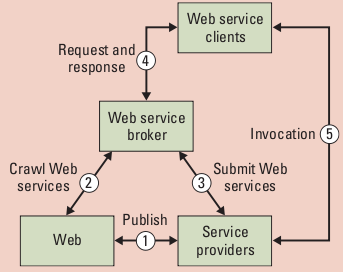
\includegraphics[scale=0.7]{images/web-service-broker.png}
	\captionof{figure}{Arquitetura do \textit{Web Service Broker} \cite{al2008toward}}
	\label{fig:web-service-broker}
\end{center}


Neste modelo, os provedores publicam informações sobre seus serviços em um diretório UDDI ou em motores de busca (passo 1). O WSB coleta informações sobre os \textit{Web Services} disseminados pela Web e continuamente monitora seus comportamentos, baseado em parâmetros de QWS (passo 2). O WSB não requer nenhuma intervenção humana, sendo totalmente automatizado. Provedores também podem submeter seus \textit{Web Services} ao WSB (passo 3). A interface do WSB permite que clientes localizem serviços, baseados em parâmetros de QWS (passo 4). Quando os clientes recebem mensagens de resposta, eles podem invocar os serviços (passo 5). É assumido que os serviços monitorados suportam invocação de operações sem cobrança de taxas ou assinaturas. A interface dos \textit{Web Services} deve suportar \textit{ping} para não sobrecarregar o sistema durante o monitoramente. O WSB realiza uma série de testes para determinar a disponibilidade de um determinado serviço, como verificar se o WSDL possui um endereço válido para um \textit{end point}.


\subsubsection{Conclusões}

O \textit{Web Service Broker} permitiu a coleta de informações sobre parâmetros de qualidade de serviço de diferentes \textit{Web Services}, que podem ser usados por instituições para busca de serviços relevantes, que atendam aos seus requisitos de qualidade de serviço.

